%!TEX TS-program = xelatex
\documentclass[notes,12pt, aspectratio=169]{beamer}

\usepackage{amsmath,amsfonts,amssymb,amsthm,mathtools}  % пакеты для математики
\usepackage{minted}

\usepackage[english, russian]{babel} % выбор языка для документа
\usepackage[utf8]{inputenc} % задание utf8 кодировки исходного tex файла
\usepackage[X2,T2A]{fontenc}        % кодировка

\usepackage{fontspec}         % пакет для подгрузки шрифтов
\setmainfont{Helvetica}  % задаёт основной шрифт документа

% why do we need \newfontfamily:
% http://tex.stackexchange.com/questions/91507/
\newfontfamily{\cyrillicfonttt}{Helvetica}
\newfontfamily{\cyrillicfont}{Helvetica}
\newfontfamily{\cyrillicfontsf}{Helvetica}

\usepackage{unicode-math}     % пакет для установки математического шрифта
% \setmathfont{Neo Euler} % шрифт для математики

\usepackage{polyglossia}      % Пакет, который позволяет подгружать русские буквы
\setdefaultlanguage{russian}  % Основной язык документа
\setotherlanguage{english}    % Второстепенный язык документа

% Шрифт для кода
\setmonofont[Scale=0.85]{Monaco}
\usepackage{verbments}

\usepackage{pgfpages}
% These slides also contain speaker notes. You can print just the slides,
% just the notes, or both, depending on the setting below. Comment out the want
% you want.
%\setbeameroption{hide notes} % Only slide
%\setbeameroption{show only notes} % Only notes
%\setbeameroption{show notes on second screen=right} % Both

\usepackage{array}

\usepackage{tikz}
\usepackage{verbatim}
\setbeamertemplate{note page}{\pagecolor{yellow!5}\insertnote}
\usetikzlibrary{positioning}
\usetikzlibrary{snakes}
\usetikzlibrary{calc}
\usetikzlibrary{arrows}
\usetikzlibrary{decorations.markings}
\usetikzlibrary{shapes.misc}
\usetikzlibrary{matrix,shapes,arrows,fit,tikzmark}

\usepackage{hyperref}
\usepackage{lipsum}
\usepackage{multimedia}
\usepackage{multirow}
\usepackage{dcolumn}
\usepackage{bbm}
\newcolumntype{d}[0]{D{.}{.}{5}}

\usepackage{changepage}
\usepackage{appendixnumberbeamer}
\newcommand{\beginbackup}{
   \newcounter{framenumbervorappendix}
   \setcounter{framenumbervorappendix}{\value{framenumber}}
   \setbeamertemplate{footline}
   {
     \leavevmode%
     \hline
     box{%
       \begin{beamercolorbox}[wd=\paperwidth,ht=2.25ex,dp=1ex,right]{footlinecolor}%
%         \insertframenumber  \hspace*{2ex} 
       \end{beamercolorbox}}%
     \vskip0pt%
   }
 }
\newcommand{\backupend}{
   \addtocounter{framenumbervorappendix}{-\value{framenumber}}
   \addtocounter{framenumber}{\value{framenumbervorappendix}} 
}

% для имитации питоновского синтаксиса 
\newcommand{\pgr}[1]{{\color{green} \textbf{#1}}}


%%%%%%%%%% Работа с картинками %%%%%%%%%
\usepackage{graphicx}                  % Для вставки рисунков
\usepackage{graphics}
\graphicspath{{images/}}    % можно указать папки с картинками
\usepackage{wrapfig}                   % Обтекание рисунков и таблиц текстом

\usepackage[space]{grffile}
\usepackage{booktabs}

% These are my colors -- there are many like them, but these ones are mine.
\definecolor{blue}{RGB}{0,114,178}
\definecolor{red}{RGB}{213,94,0}
\definecolor{yellow}{RGB}{240,228,66}
\definecolor{green}{RGB}{0,128, 0}

\hypersetup{
  colorlinks=false,
  linkbordercolor = {white},
  linkcolor = {blue}
}


%% I use a beige off white for my background
\definecolor{MyBackground}{RGB}{255,253,218}

%% Uncomment this if you want to change the background color to something else
%\setbeamercolor{background canvas}{bg=MyBackground}

%% Change the bg color to adjust your transition slide background color!
\newenvironment{transitionframe}{
  \setbeamercolor{background canvas}{bg=yellow}
  \begin{frame}}{
    \end{frame}
}

\setbeamercolor{frametitle}{fg=blue}
\setbeamercolor{title}{fg=black}
\setbeamertemplate{footline}[frame number]
\setbeamertemplate{navigation symbols}{} 
\setbeamertemplate{itemize items}{-}
\setbeamercolor{itemize item}{fg=blue}
\setbeamercolor{itemize subitem}{fg=blue}
\setbeamercolor{enumerate item}{fg=blue}
\setbeamercolor{enumerate subitem}{fg=blue}
\setbeamercolor{button}{bg=MyBackground,fg=blue,}


% If you like road maps, rather than having clutter at the top, have a roadmap show up at the end of each section 
% (and after your introduction)
% Uncomment this is if you want the roadmap!
% \AtBeginSection[]
% {
%    \begin{frame}
%        \frametitle{Roadmap of Talk}
%        \tableofcontents[currentsection]
%    \end{frame}
% }
\setbeamercolor{section in toc}{fg=blue}
\setbeamercolor{subsection in toc}{fg=red}
\setbeamersize{text margin left=1em,text margin right=1em} 

% списки, которые растягиваются на всю величину слайда 
\newenvironment{wideitemize}{\itemize\addtolength{\itemsep}{10pt}}{\enditemize}



\title[]{\textcolor{blue}{Практический анализ данных и машинное обучение: искусственные нейронные сети}}
\author{Ульянкин Филипп, Соловей Влад}
\date{\today}


\begin{document}

%%% TIKZ STUFF
\tikzset{   
        every picture/.style={remember picture,baseline},
        every node/.style={anchor=base,align=center,outer sep=1.5pt},
        every path/.style={thick},
        }
\newcommand\marktopleft[1]{%
    \tikz[overlay,remember picture] 
        \node (marker-#1-a) at (-.3em,.3em) {};%
}
\newcommand\markbottomright[2]{%
    \tikz[overlay,remember picture] 
        \node (marker-#1-b) at (0em,0em) {};%
}
\tikzstyle{every picture}+=[remember picture] 
\tikzstyle{mybox} =[draw=black, very thick, rectangle, inner sep=10pt, inner ysep=20pt]
\tikzstyle{fancytitle} =[draw=black,fill=red, text=white]
%%%% END TIKZ STUFF

% Title Slide
\begin{frame}
\maketitle
\centering Transfer learning 
\end{frame}


\begin{frame}{Agenda} 
\begin{wideitemize}
	\item Transfer learning 
	\item Локализация
	\item Сегментация  
\end{wideitemize}
\end{frame}


\begin{transitionframe}
	\begin{center}
		\Huge Transfer learning
	\end{center}
\end{transitionframe}


	\begin{frame}{Что выучивают нейросети}
\begin{center}
	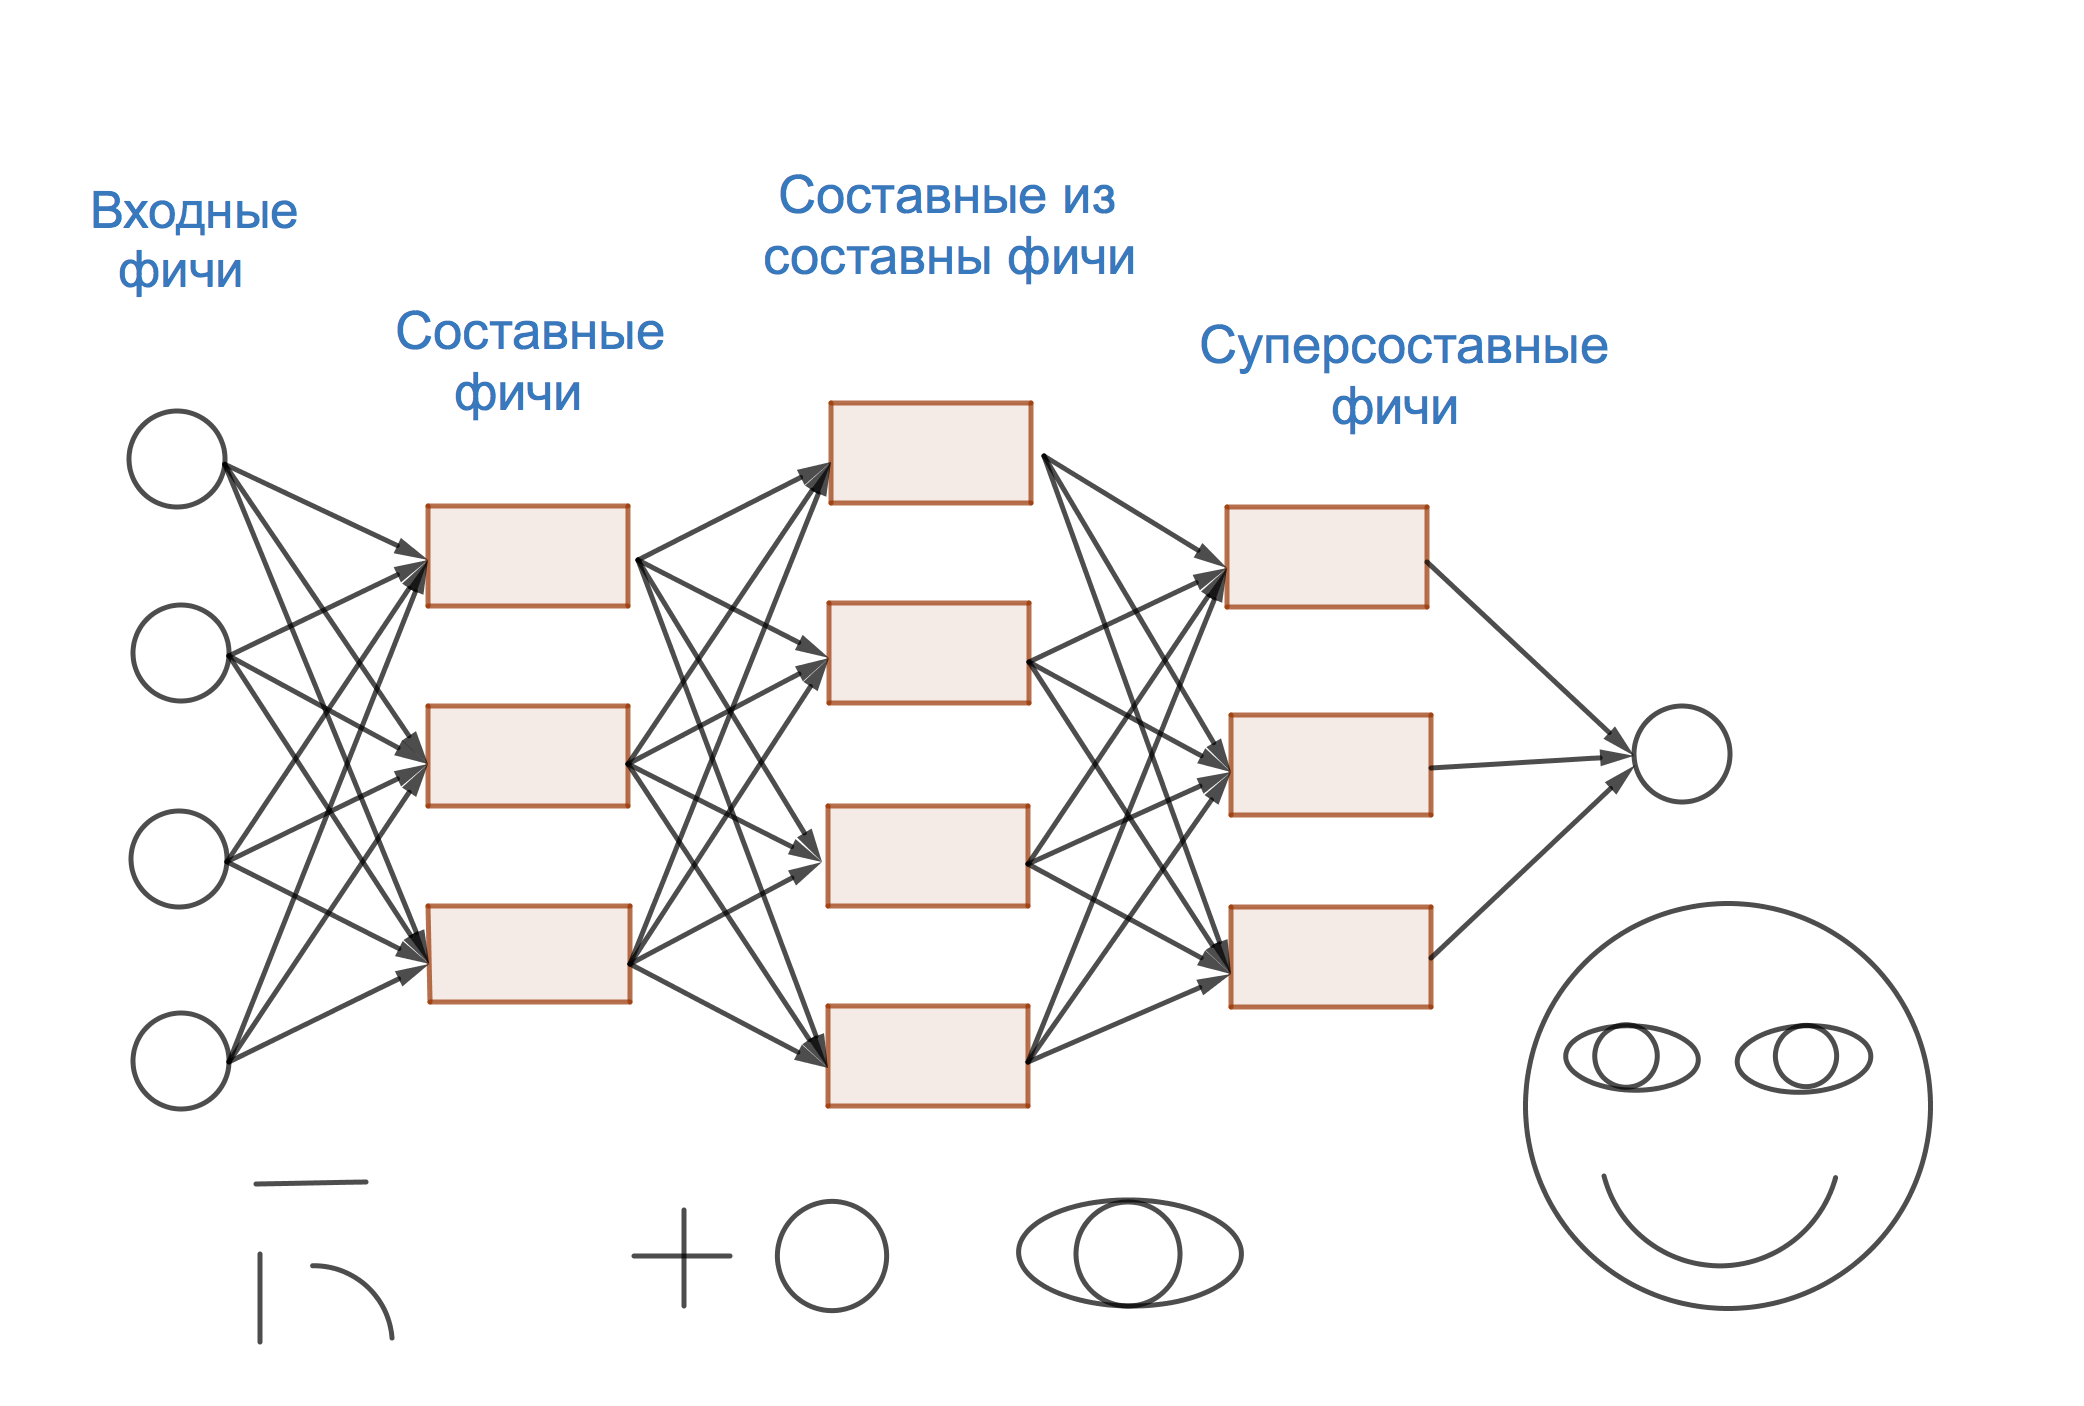
\includegraphics[width=0.73\paperwidth]{network_1.png}
\end{center}
\end{frame}


\begin{frame}{Что выучивают нейросети}
\begin{center}
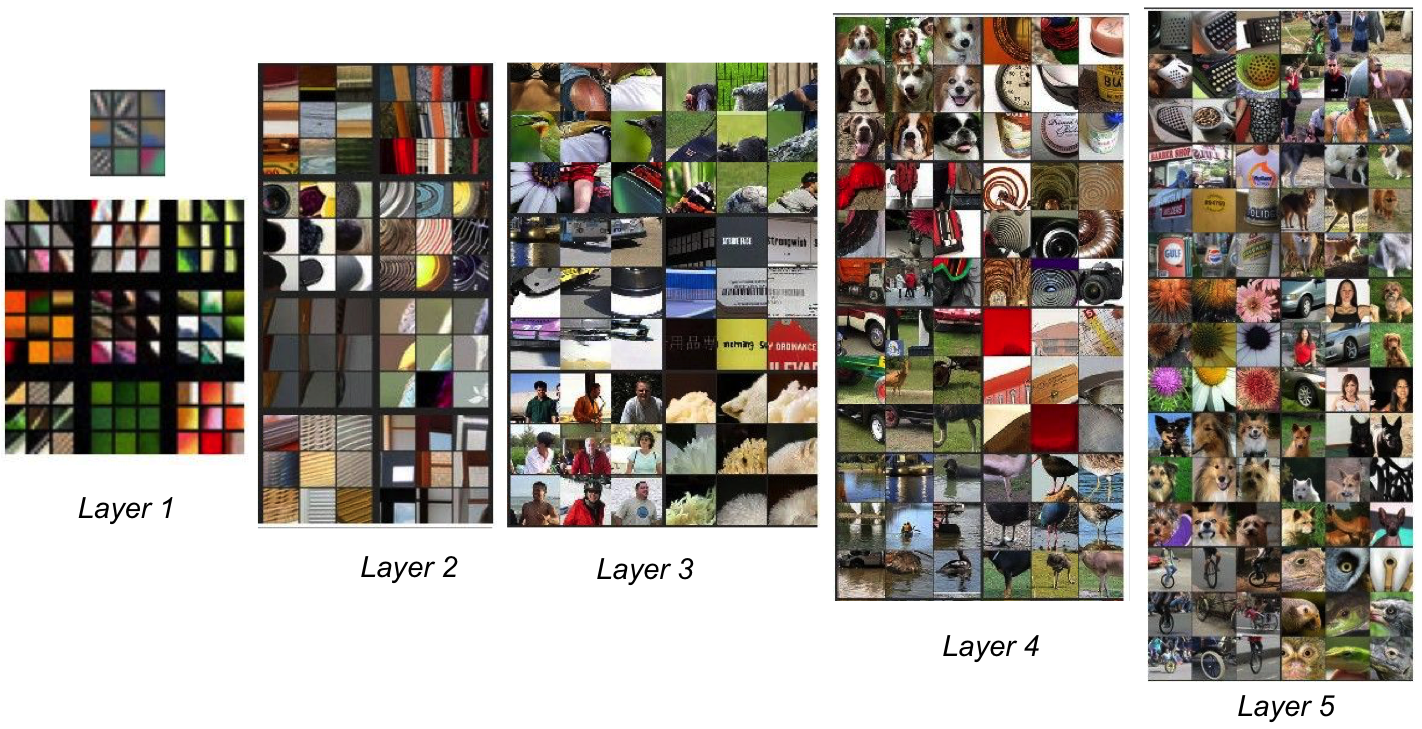
\includegraphics[width=.9\linewidth]{cnn_vis.png}
\end{center}
\vfill 
\small{\url{https://arxiv.org/pdf/1311.2901.pdf}}
\end{frame}


\begin{frame}{Transfer learning}
\begin{wideitemize}
	\item  Глубокие сети извлекают из изображений сложные фичи, но для их обучения нужно много данных...
\end{wideitemize}

\begin{center}
	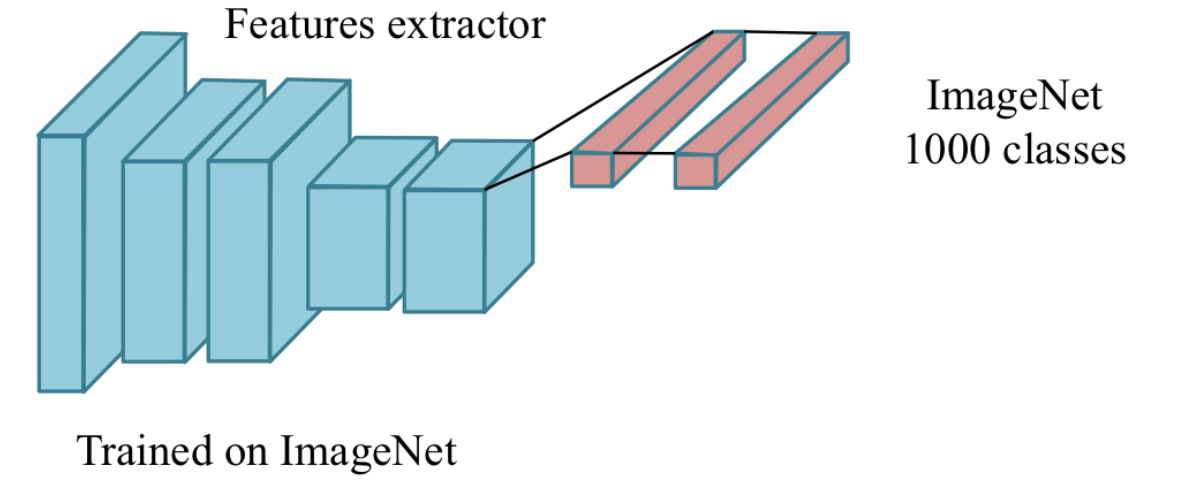
\includegraphics[width=.8\linewidth]{transfer_learning1.png}
\end{center}
\end{frame}


\begin{frame}{Transfer learning}
\begin{wideitemize}
	\item  Глубокие сети извлекают из изображений сложные фичи, но для их обучения нужно много данных...
	\item  Давайте повторно использовать уже предобученную сеть!
\end{wideitemize}

\begin{center}
	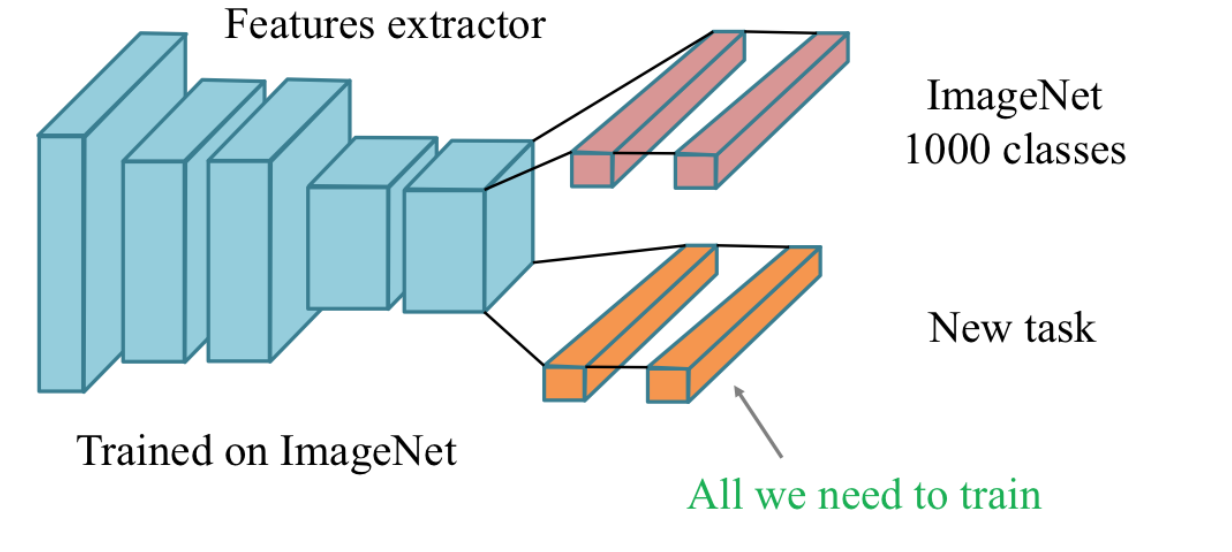
\includegraphics[width=.8\linewidth]{transfer_learning2.png}
\end{center}
\end{frame}


\begin{frame}{Transfer learning}
\begin{wideitemize}
	\item  Нужно меньше данных для обучения, так как нас интересуют лишь последние слои
	\item  Это работает если наша задача похожа на ту, для которой обучалась используемая сетка
	\item  Например, если мы хотим распознавать эмоции, в датасете для нашей сетки должны были быть человеческие лица
\end{wideitemize}
\end{frame}


\begin{frame}{Transfer learning}
\begin{center}
	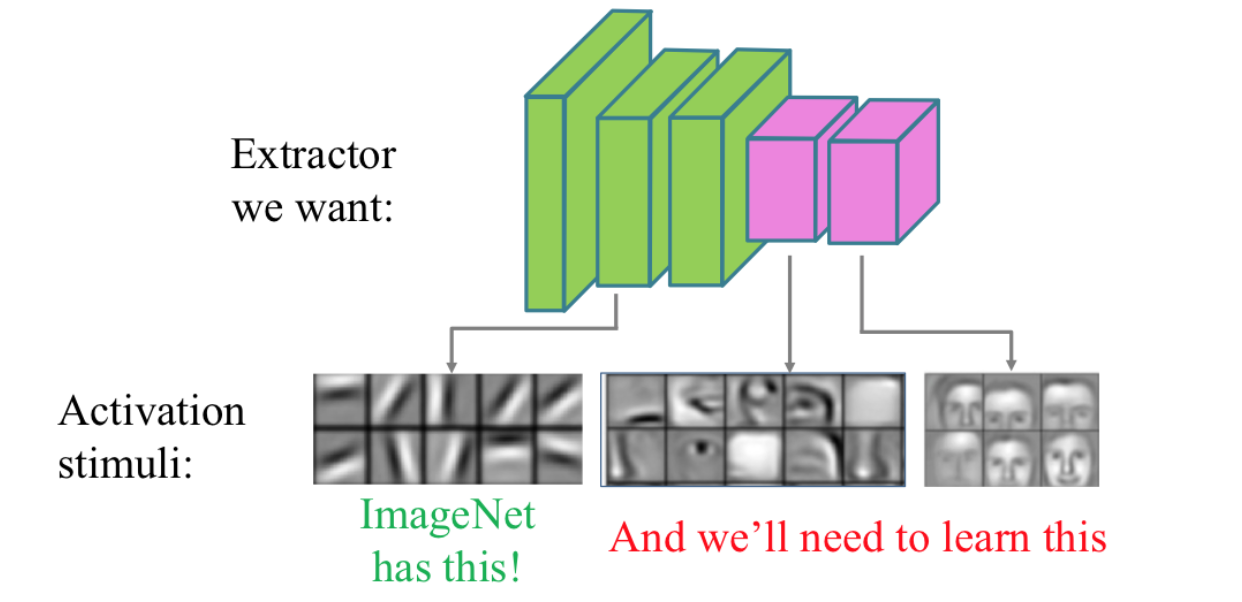
\includegraphics[width=.8\linewidth]{transfer_learning3.png}
\end{center}
\end{frame}


\begin{frame}{Transfer learning}
\begin{center}
	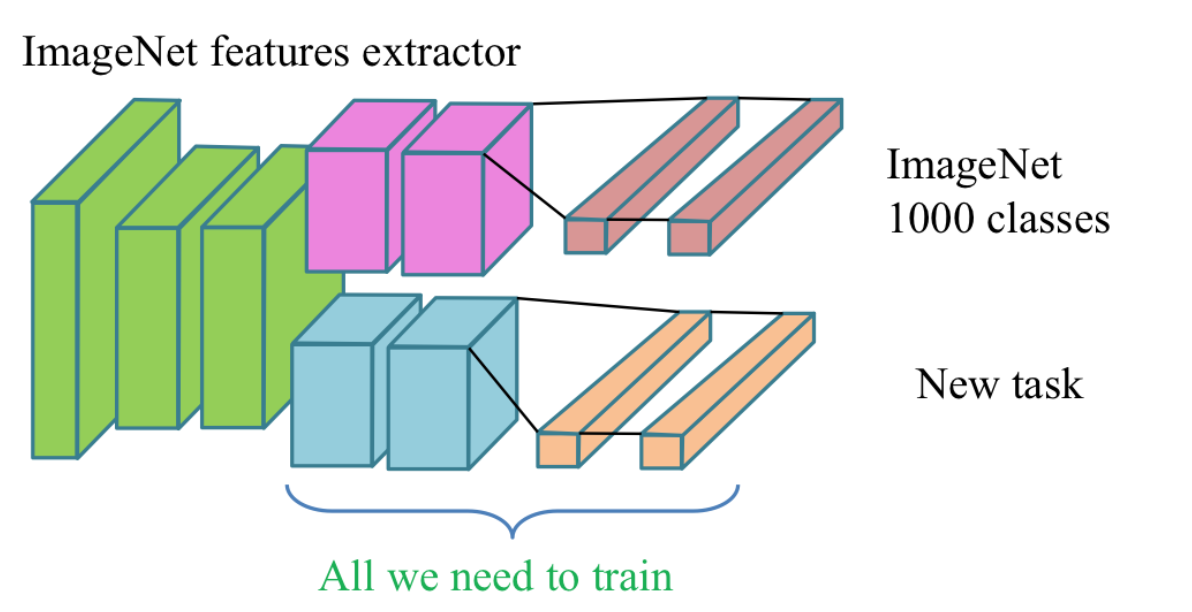
\includegraphics[width=.8\linewidth]{transfer_learning4.png}
\end{center}
\end{frame}

\begin{frame}{Крокодил learning}
\begin{center}
	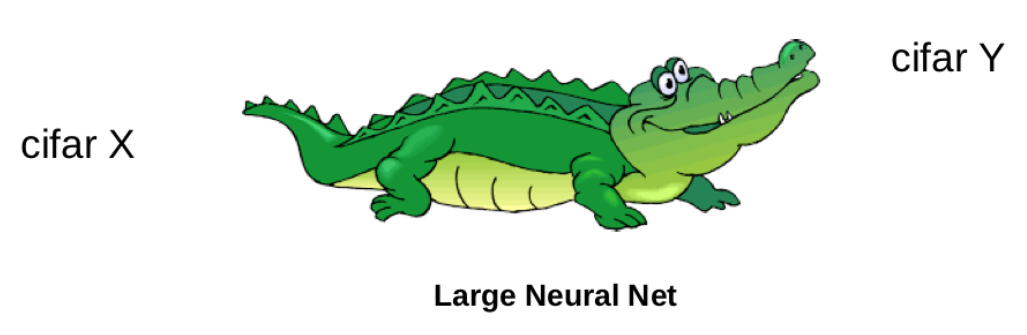
\includegraphics[width=.8\linewidth]{croc_1.png}
\end{center}
\end{frame}

\begin{frame}{Крокодил learning}
\begin{center}
	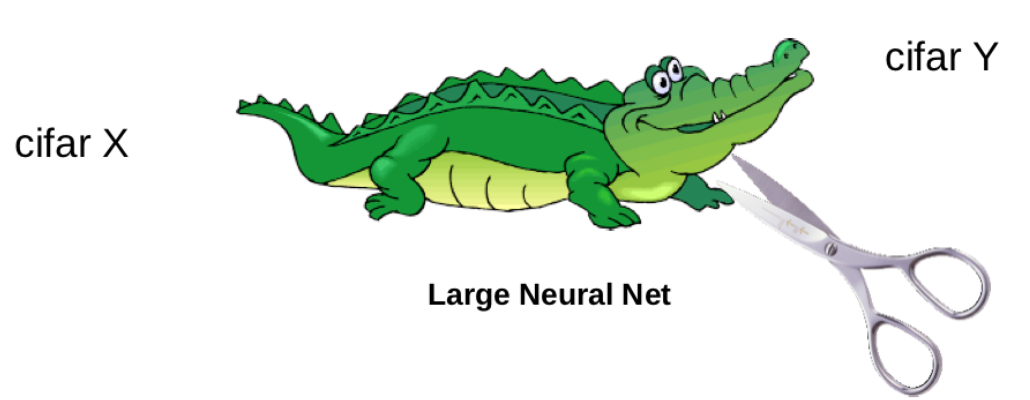
\includegraphics[width=.8\linewidth]{croc_2.png}
\end{center}
\end{frame}

\begin{frame}{Крокодил learning}
\begin{center}
	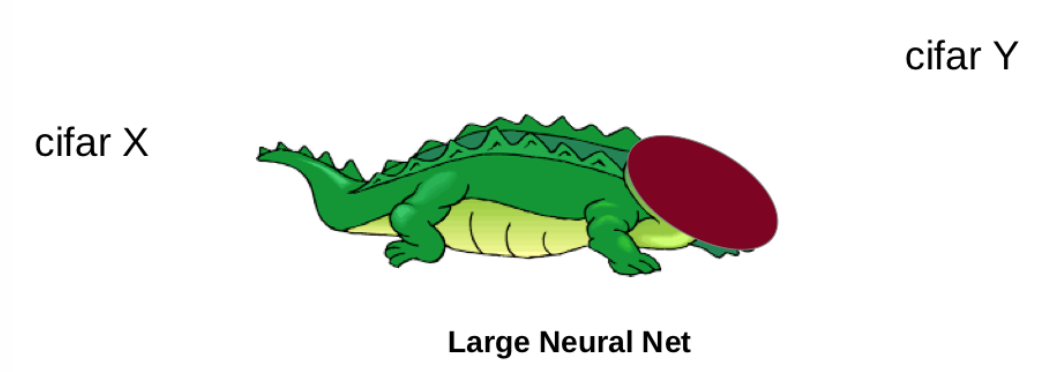
\includegraphics[width=.8\linewidth]{croc_3.png}
\end{center}
\end{frame}

\begin{frame}{Крокодил learning}
\begin{center}
	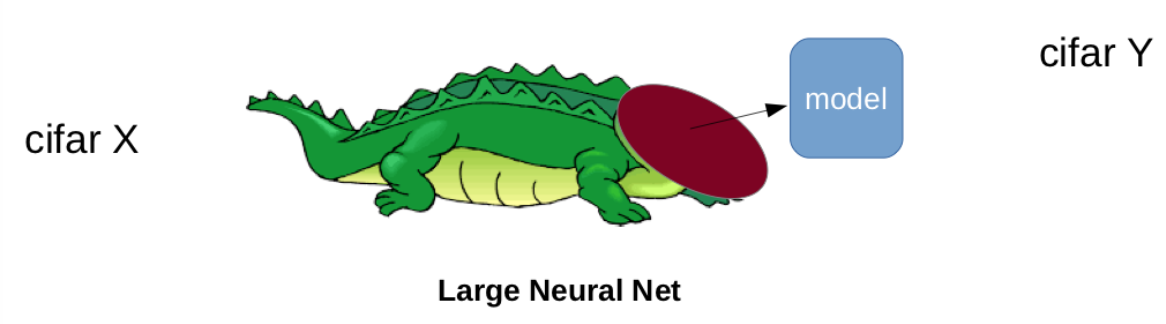
\includegraphics[width=.8\linewidth]{croc_4.png}
\end{center}
\end{frame}

\begin{frame}{Крокодил learning}
\begin{center}
	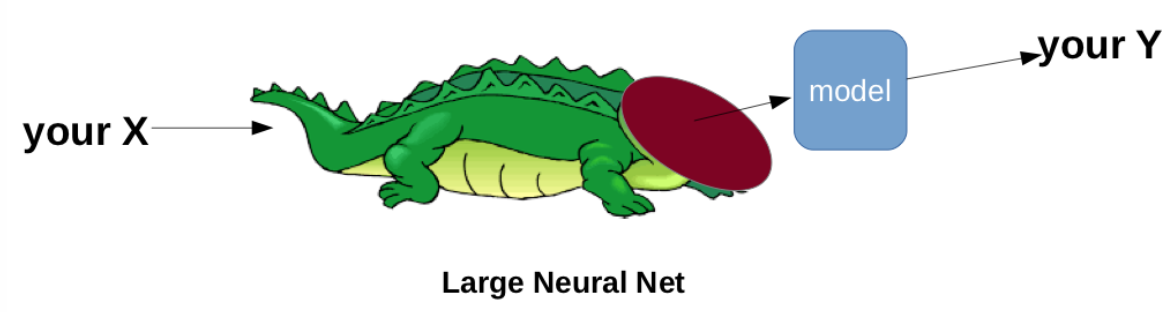
\includegraphics[width=.8\linewidth]{croc_5.png}
\end{center}
\end{frame}

\begin{frame}{Крокодил learning}
\begin{wideitemize}
	\item Отрезали у крокодила голову
	\item  Используем тело крокодила как экстрактор фичей
	\item  Вместо головы крокодила можно прикрепить что угодно 
	\item  Даже случайный лес
	\item В экстракторе фичей веса модели обычно не дообучают, дообучение касается только новой головы крокодила
\end{wideitemize}
\end{frame}

\begin{frame}{Крокодил learning}
\begin{center}
	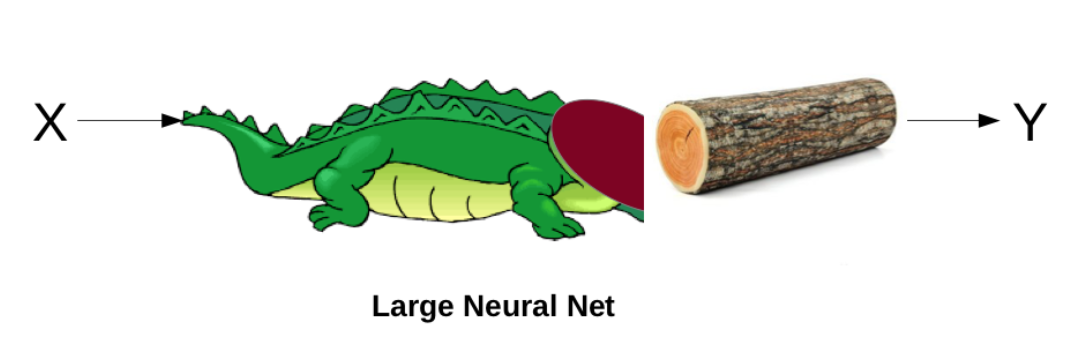
\includegraphics[width=.8\linewidth]{croc_6.png}
\end{center}
\end{frame}


\begin{transitionframe}
	\begin{center}
		\Huge Собираем своего крокодила! 
	\end{center}
\end{transitionframe}


\begin{frame}{Зоопарки моделей}
\begin{wideitemize}
	\item Перед тем как решать задачу, убедитесь, что уже нет решения и вы не можете его украсть
	\item Один из зоопарков моделей: {\color{blue} \url{https://github.com/BVLC/caffe/wiki/Model-Zoo}}
	\item Ещё зоопарк: {\color{blue} \url{ https://modelzoo.co}}
\end{wideitemize}
\end{frame}


 \begin{transitionframe}
	\begin{center}
		\Huge  Сегментация изображения
	\end{center}
\end{transitionframe}


\begin{frame}{Сегментация и локализация}
\begin{center}
	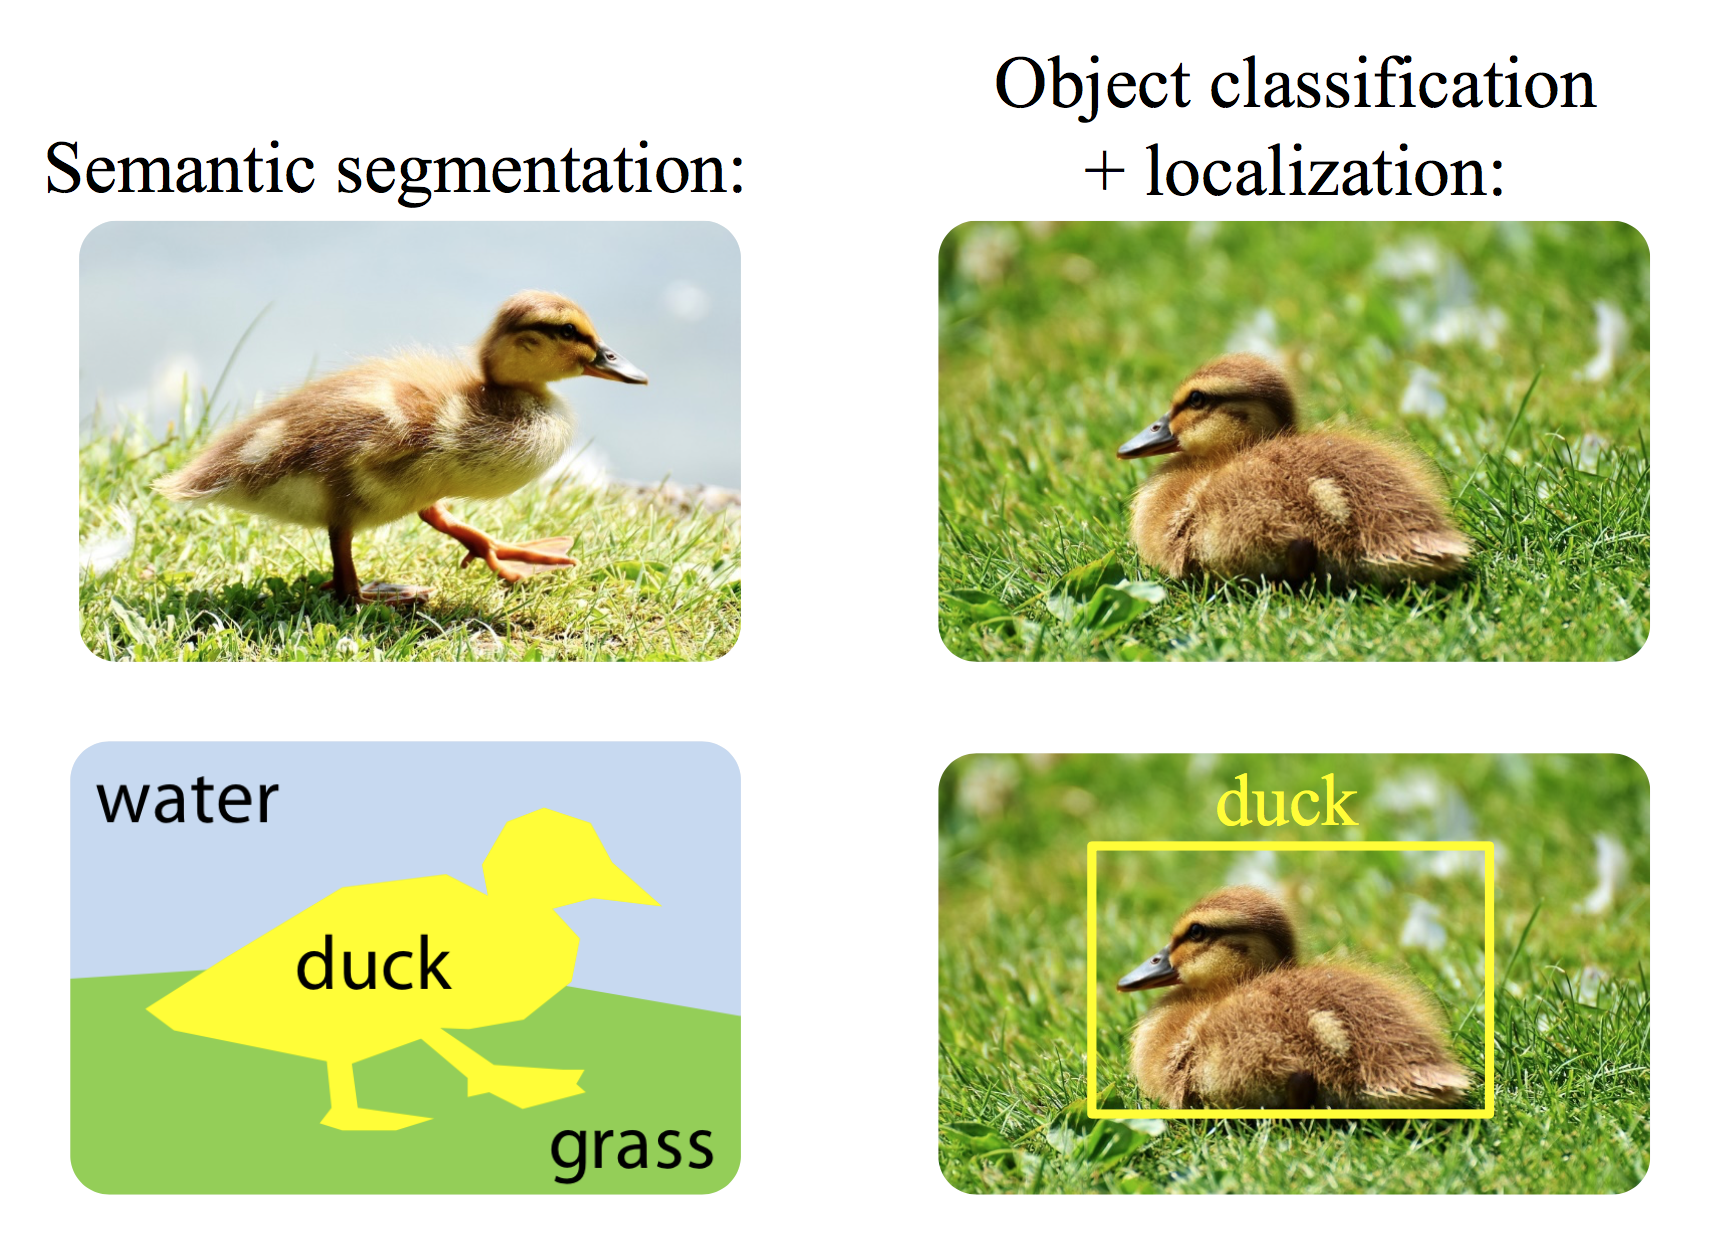
\includegraphics[width=.7\linewidth]{duck.png}
\end{center}
\end{frame}


\begin{frame}{Сегментация}
\begin{center}
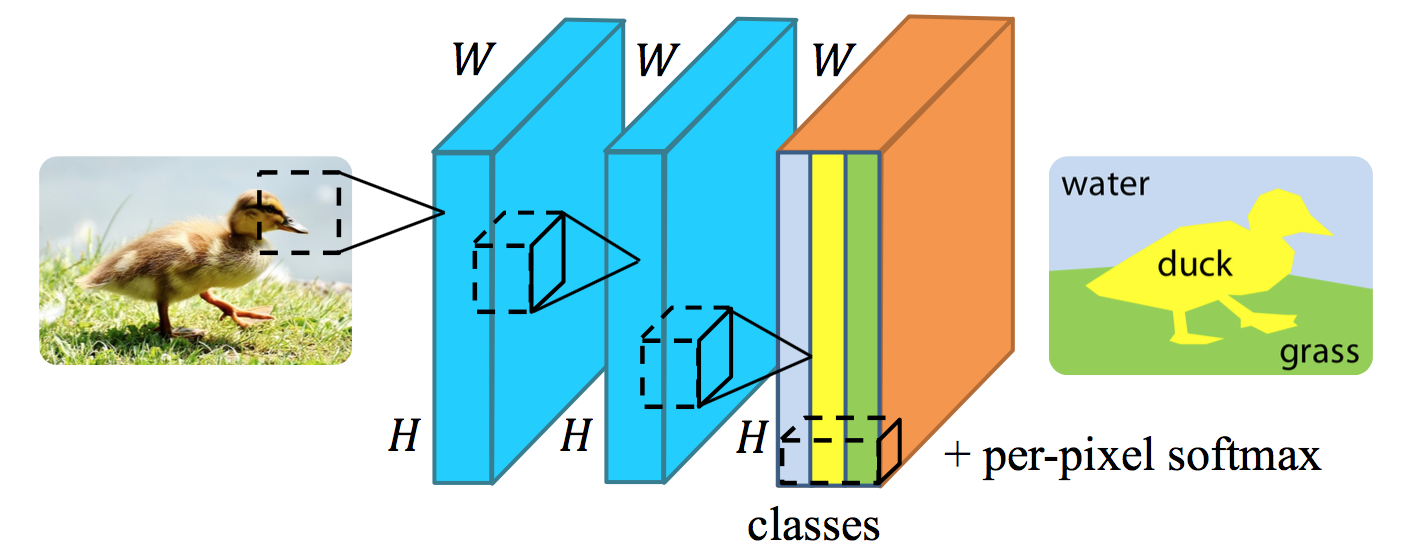
\includegraphics[width=.9\linewidth]{duck_1.png}
\end{center}
\begin{wideitemize}
\item Нам нужно научиться классифицировать каждый пиксель
\item Куча свёрток и попиксельный softmax 
\end{wideitemize}
\end{frame}


\begin{frame}{Сегментация}
\begin{center}
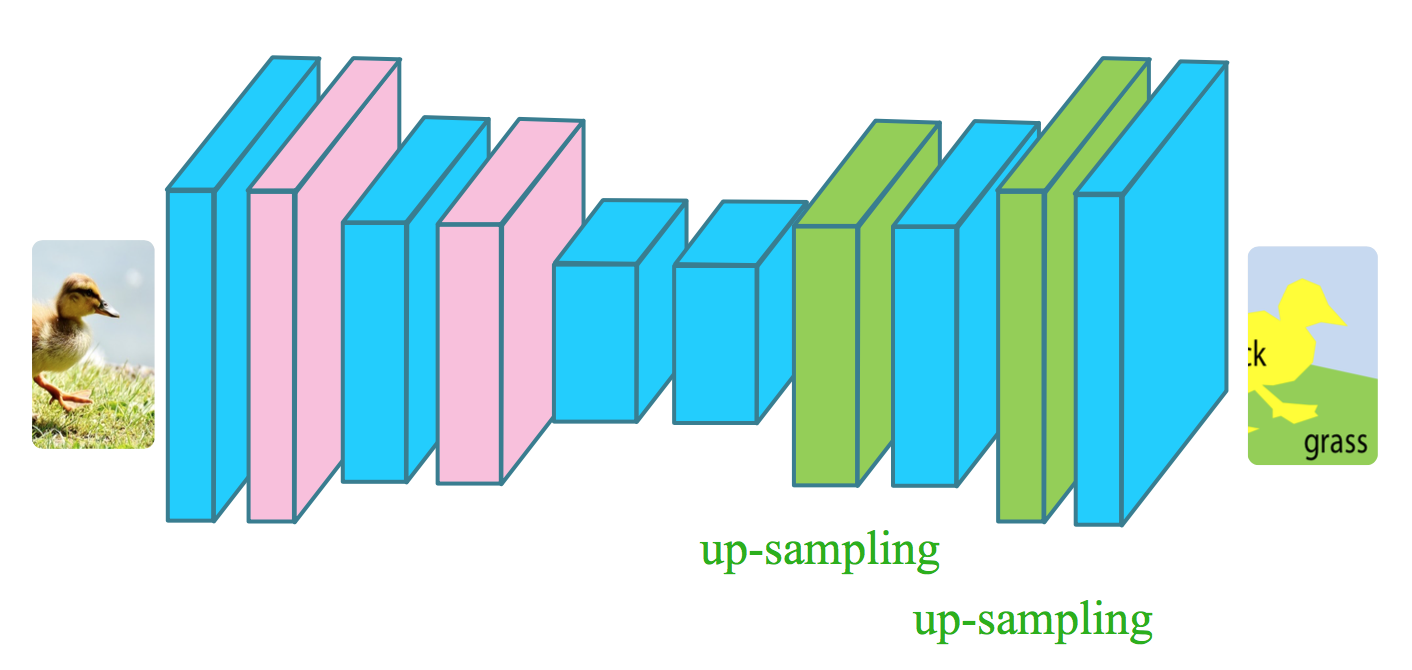
\includegraphics[width=.8\linewidth]{duck_2.png}
\end{center}
\begin{itemize}
\item Если захотим добавить пулинг, придётся делать анпулинг
\item Подобную технику мы уже видели в автокодировщиках 
\end{itemize}
\end{frame}


\begin{frame}{Nearest neighbor unpooling}
\begin{center}
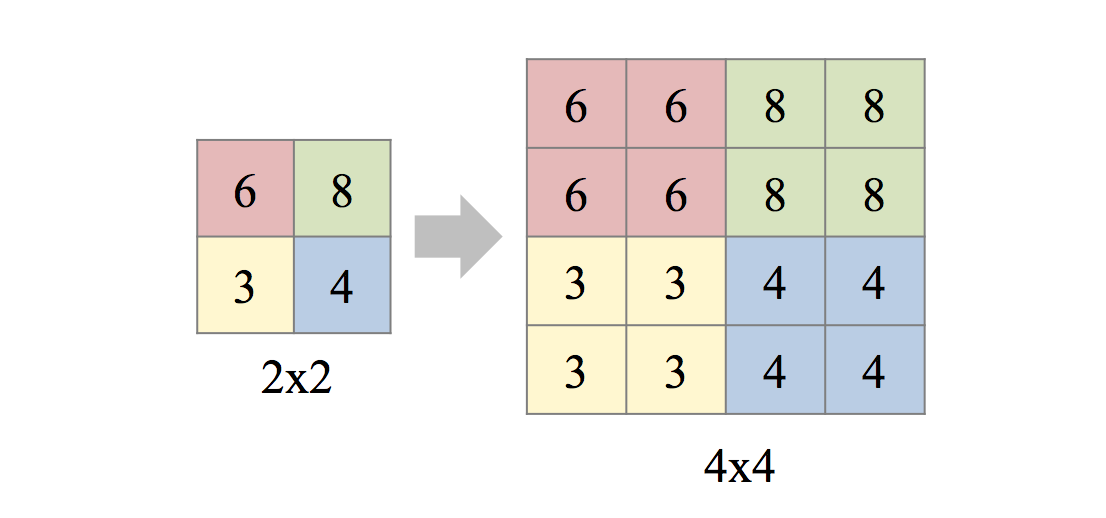
\includegraphics[width=.9\linewidth]{nnun.png}
\end{center}
\end{frame}


\begin{frame}{Max unpooling}
\begin{center}
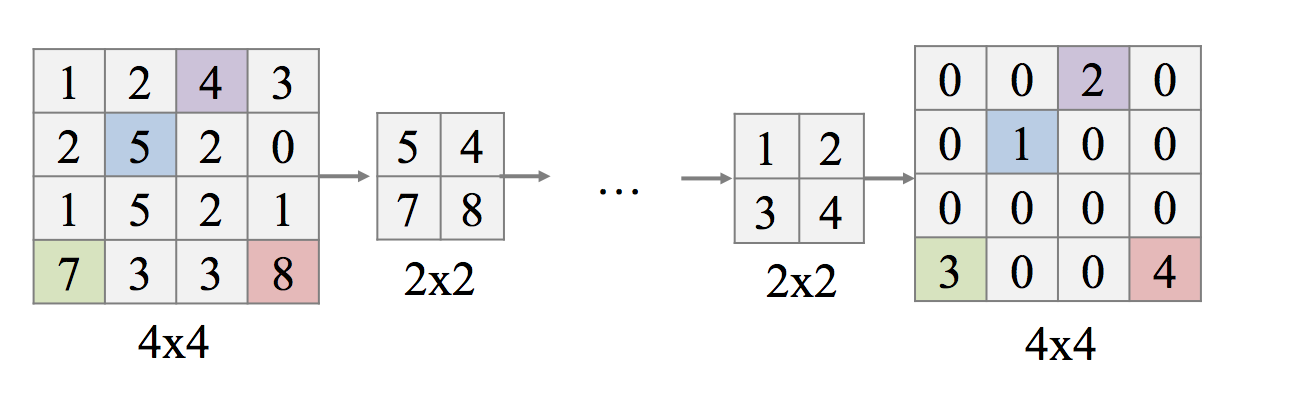
\includegraphics[width=.9\linewidth]{maxun.png}
\end{center}
\end{frame}


\begin{frame}{Learnable unpooling}
\begin{center}
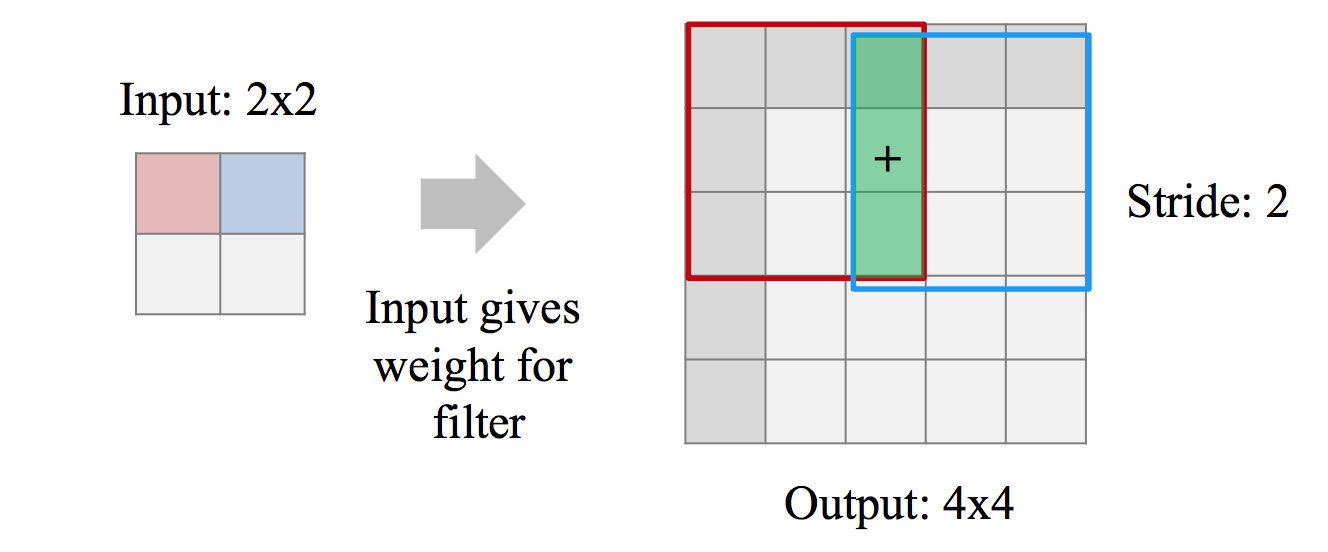
\includegraphics[width=.9\linewidth]{leun.png}
\end{center}
\end{frame}


\begin{frame}{Примеры}
\begin{center}
	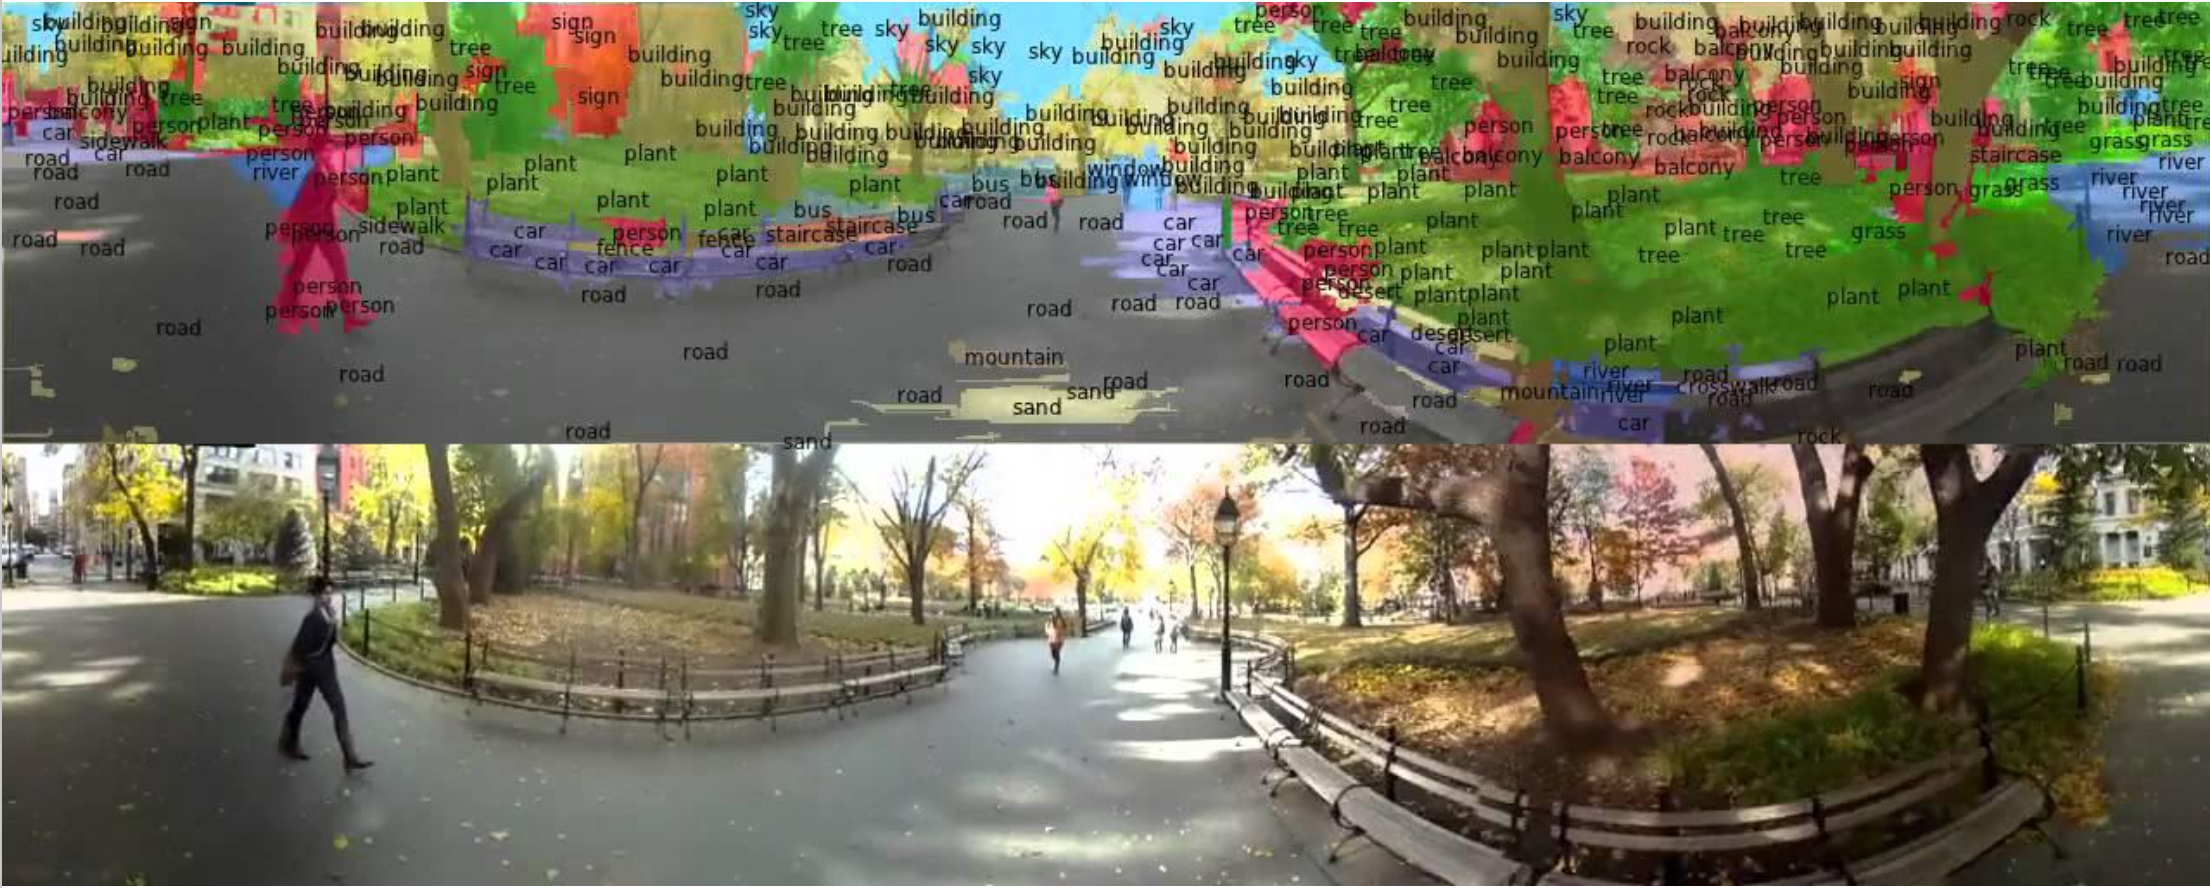
\includegraphics[width=.9\linewidth]{seg.png}
\end{center}
\url{https://www.youtube.com/watch?v=ZJMtDRbqH40}
\end{frame}


\begin{frame}{Fully-convolution net}
\begin{center}
	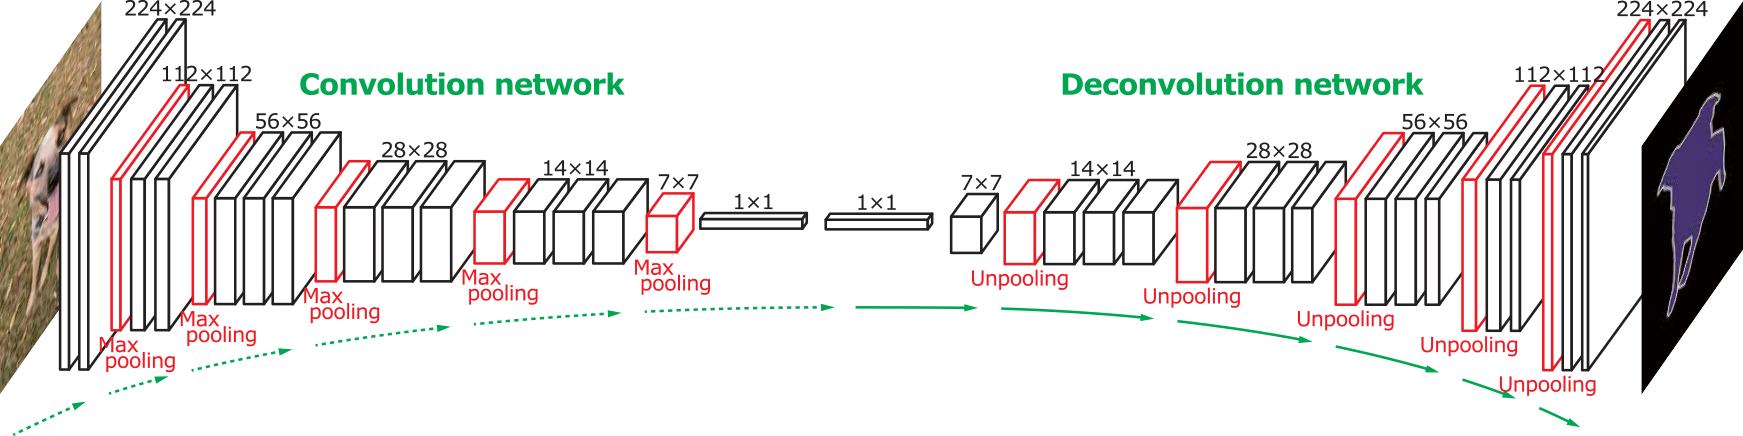
\includegraphics[width=.8\linewidth]{fully_net.png}
\end{center}
\begin{itemize}
	\item Cвернули в скрытое представление, развернули, спрогнозировали
\end{itemize}
\end{frame}


\begin{frame}{U-net}
\begin{center}
	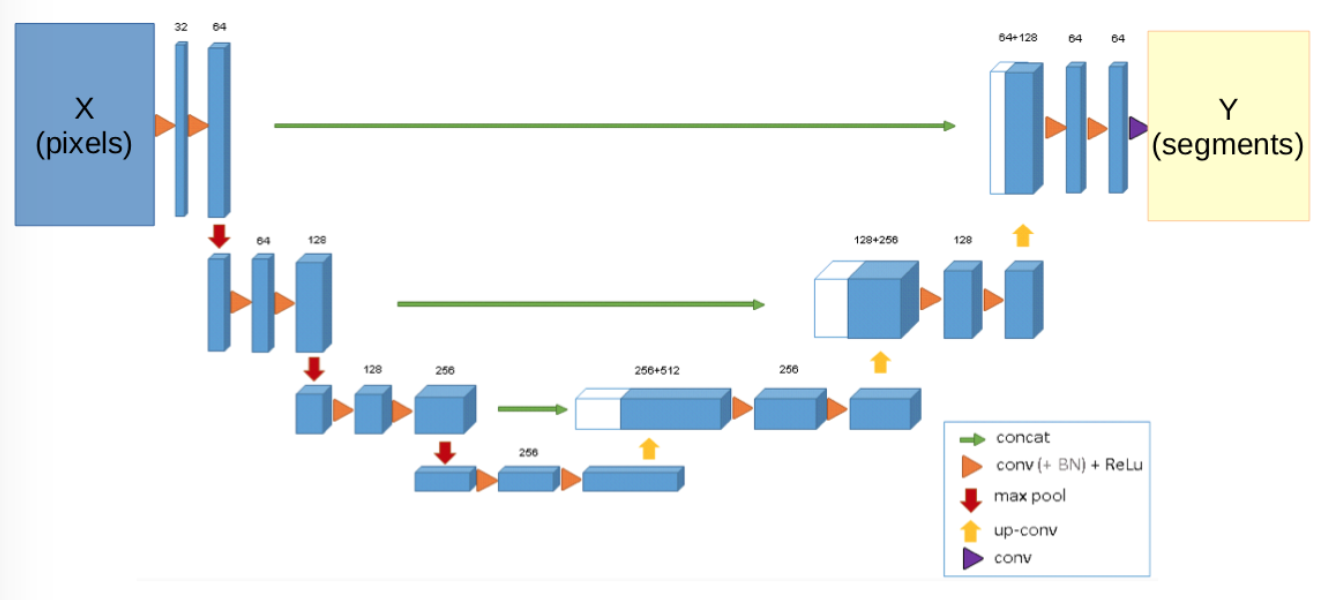
\includegraphics[width=.8\linewidth]{unet.png}
\end{center}
\begin{itemize}
	\item Можно добавить связи между слоями, отражающими одинаковую абстракцию, это должно улучшить модель
\end{itemize}
\end{frame}


 \begin{transitionframe}
	\begin{center}
		\Huge  Локализация изображения
	\end{center}
\end{transitionframe}


\begin{frame}{Локализация}
\begin{center}
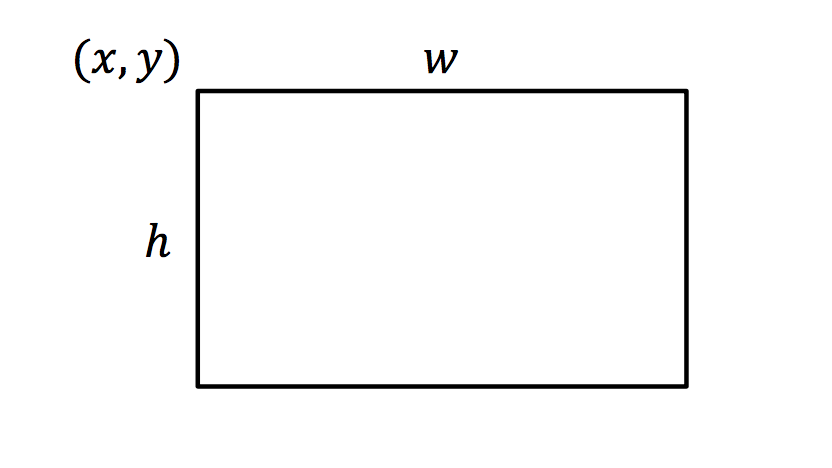
\includegraphics[width=.5\linewidth]{box.png}
\end{center}
\begin{wideitemize}
\item для локализации объекта нужно нащупать рамочку, в котором он находится
\item рамочка описывается параметрами $(x,y,w,h)$
\end{wideitemize}
\end{frame}


\begin{frame}{Локализация}
\begin{center}
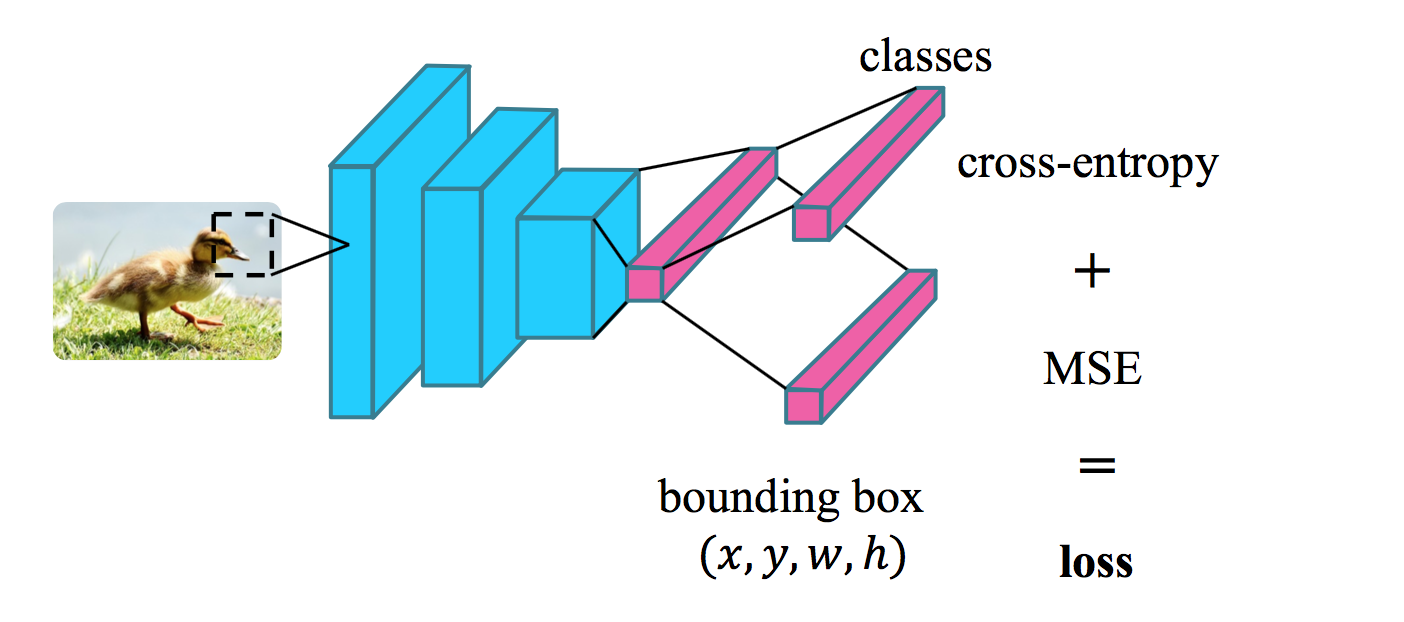
\includegraphics[width=.9\linewidth]{duck_3.png}
\end{center}
\end{frame}


\begin{frame}{Примеры}
\begin{center}
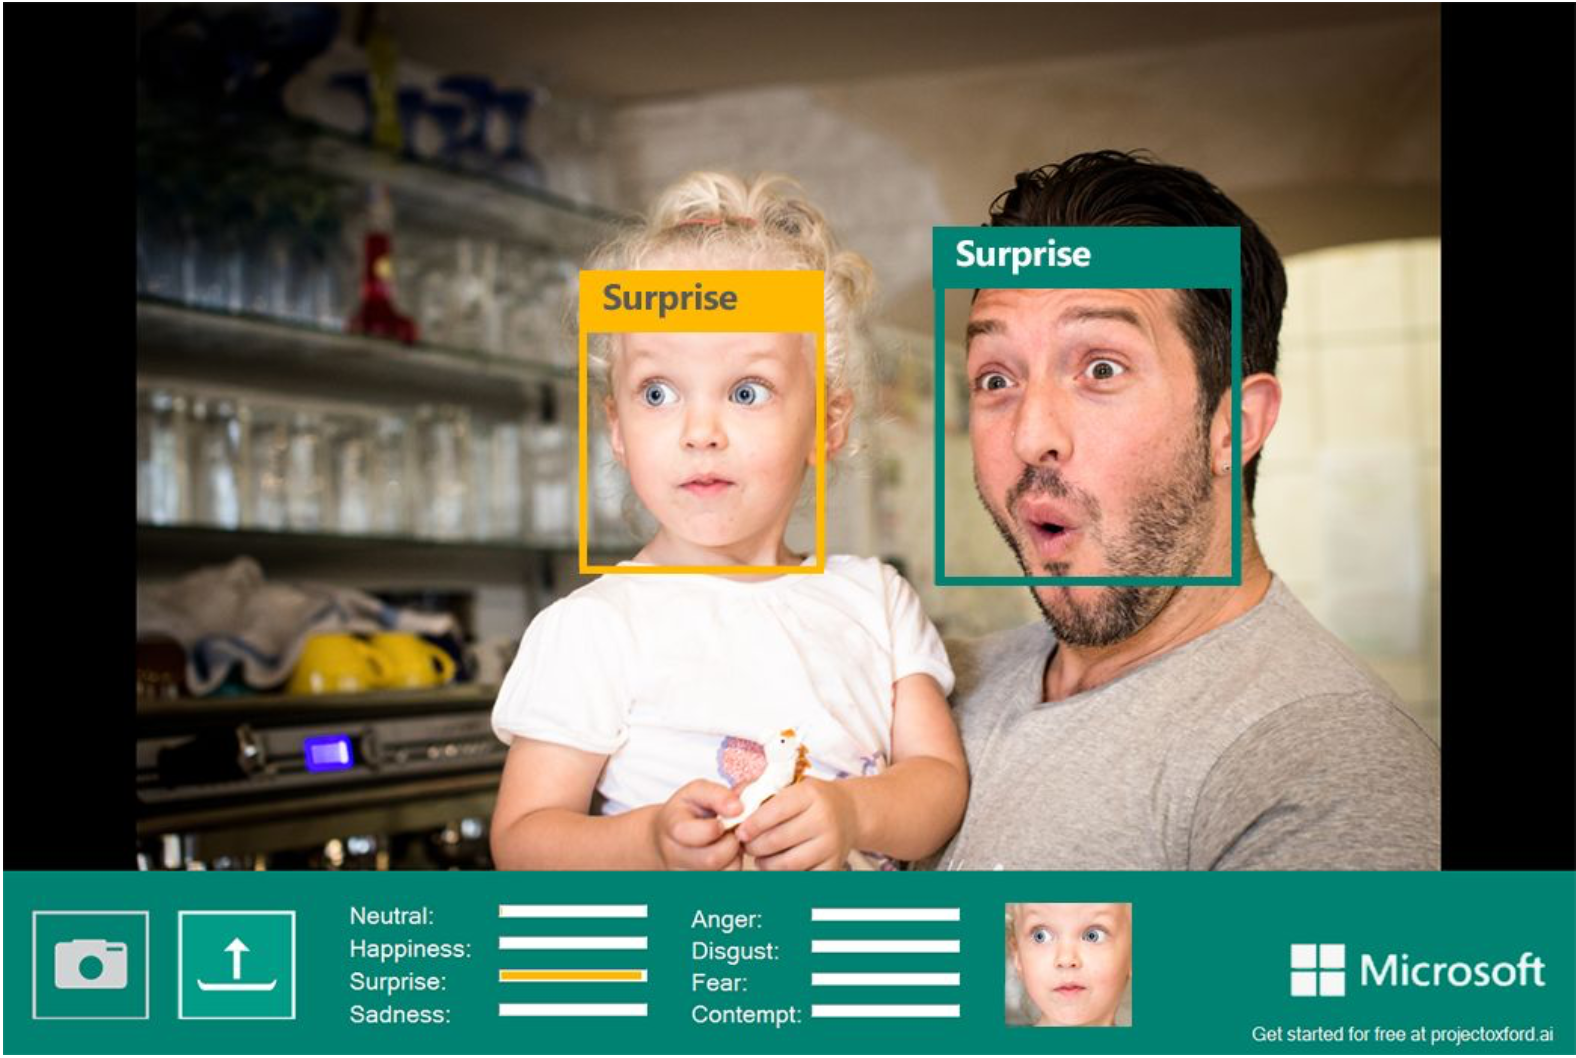
\includegraphics[width=.7\linewidth]{loc1.png}
\end{center}
\end{frame}


\begin{frame}{Примеры}
\begin{center}
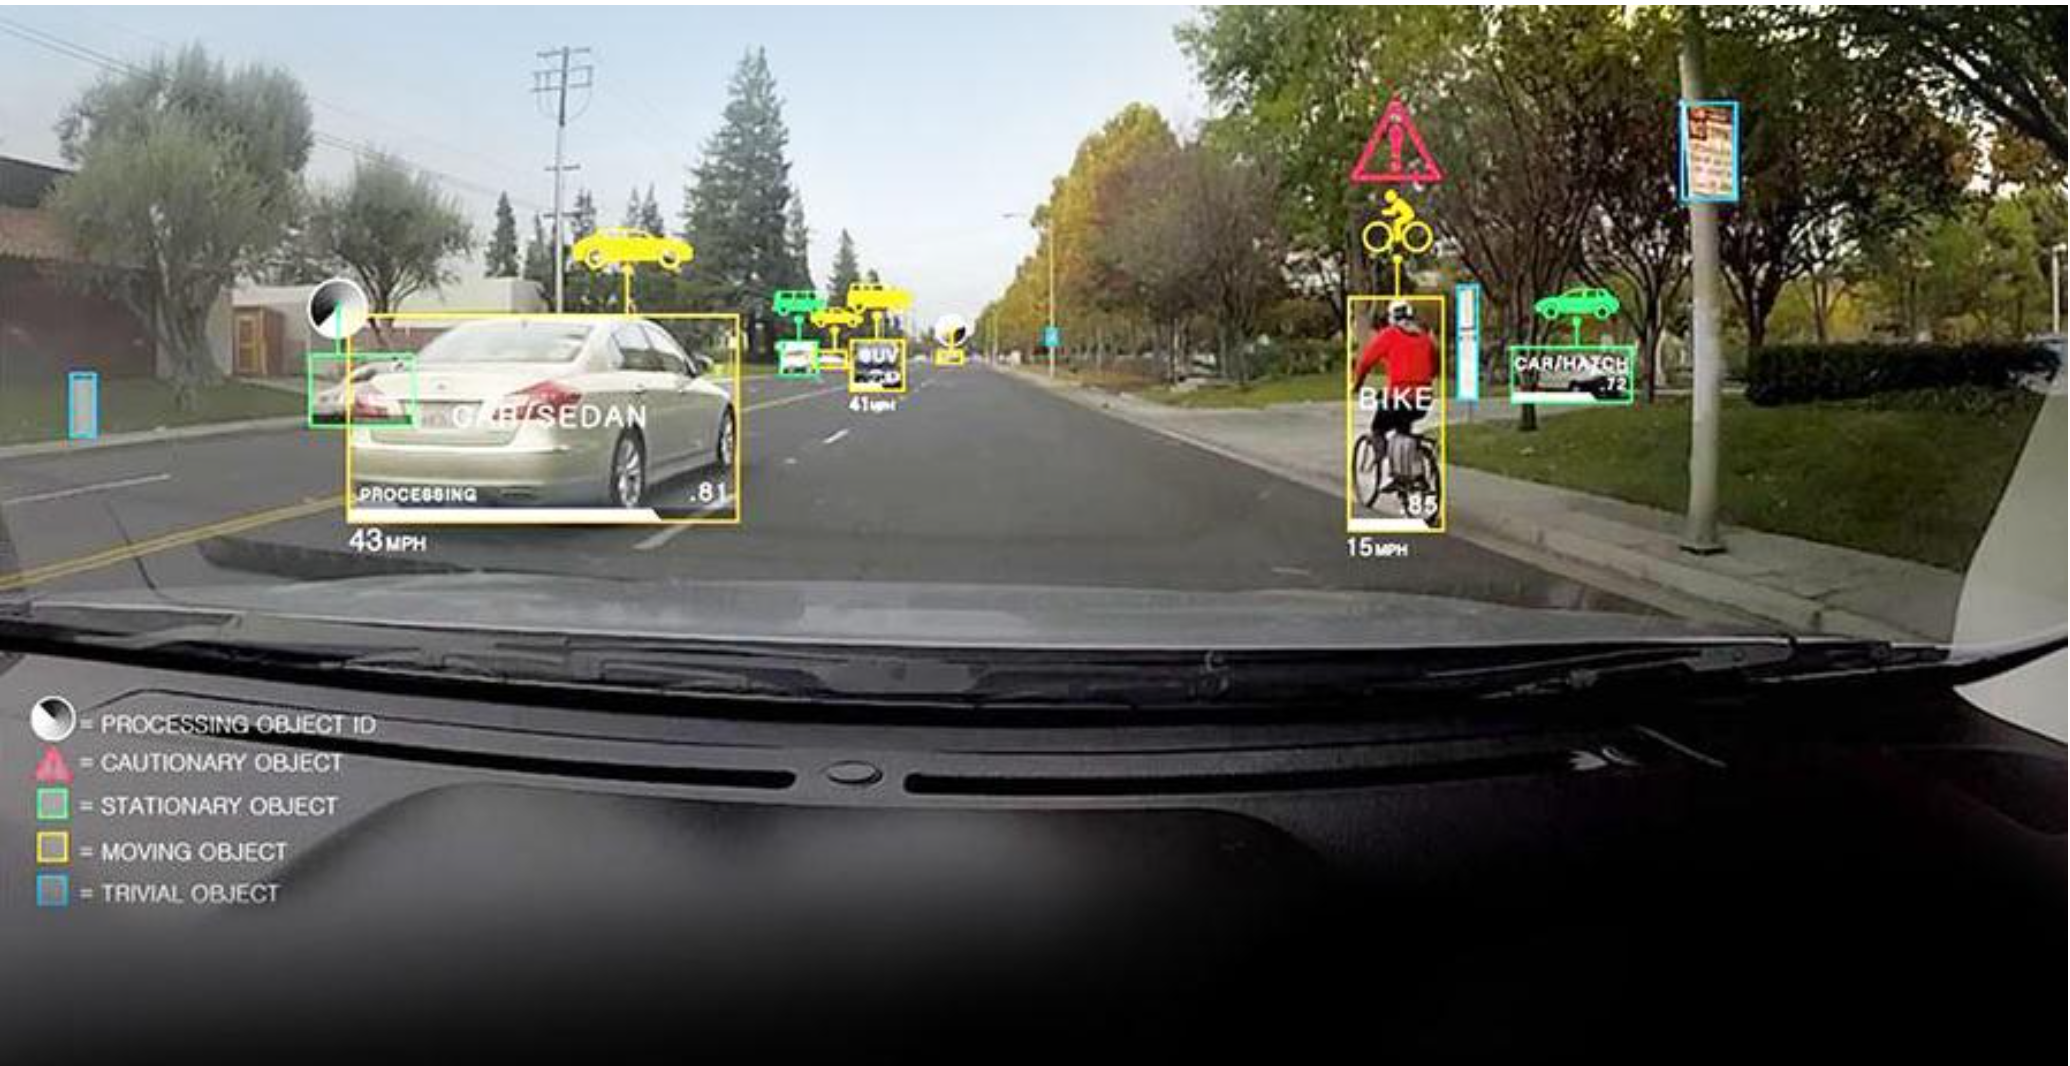
\includegraphics[width=.9\linewidth]{loc2.png}
\end{center}
\end{frame}


\begin{transitionframe}
	\begin{center}
		\Huge Собираем fully connected net и U-net!
	\end{center}
\end{transitionframe}

\end{document}
